\chapter{Escalation to Human Experts}\label{chap:escalation}

The techniques presented in the previous chapters allow WCA applications to
detect states that the developer trains models to handle.
The developer can provide example images of the object after each step has been
done correctly.
However, there are many possible ways that an object can be put together
incorrectly.
It is not possible to collect images of every mistake that someone completing a
task might make.
People using these
applications in the real world are going to reach some states that the models
were not trained for. As Dr. Reynold Xin once said,
``A machine learning model is only as good as the data it is fed~\cite{xin}.''
Our models can signal to our application that an image ``looks most similar to
this set of images from the training data.''
These models are not capable of a more general understanding, such as ``the long
brass piece is screwed on upside down.''

Detecting all possible error states would require us to have examples of these
states in our training data. There is a combinatorial explosion in the number of
error states, compared to the number of correct states, so collecting training
data for every possible error is not practical.
Instead, our applications handle errors by connecting the person completing the
task to a human who is an expert on this task.

% \section{Related Work}

% Microsoft Dynamics 365 Remote Assist~\cite{dynamics365} lets a human task expert
% walk someone through every step of a task. This is done remotely with the help
% of a headset, but the expert must help the person one on one, through the
% entire task.
% A task expert's time is valuable.
% We believe that integrating wearable cognitive assistance with
% human assistance will allow products like Microsoft's to scale from requiring
% experts to work one on one through each step of the task to enabling experts to
% help multiple users concurrently.

\section{Calls With Human Experts}

The computer vision models that our applications use are not perfect. In order
to handle cases where a model makes a mistake, our applications allow the user
to start a call with a human who is an expert on the task being completed. The
human expert sees a feed from the user's camera and they can talk the user
through correcting problems. In addition, the expert can change the step that
the application thinks the user is in the middle of, and then the user can
continue to receive guidance from the application after the call ends.

Computer vision models can recognize objects that they have been trained on.
When we train models for Gabriel applications, we consider each state of a task
to be one object. Open World Object Detection~\cite{joseph2021open} is an active
area of research into models that can learn to detect previously unlabeled
objects. However, this does not help with recognizing such an object the first
time it is seen. Gabriel applications need to handle all errors, even ones that
have not been seen before. A human who is an expert on the task can do this.

Correcting error states in Gabriel applications can be done on the order of tens
of seconds to a few
minutes, unlike driving a car which might require sub-second response times.
It's perfectly acceptable for the user to press a button to call for help from
an expert, if the application does not detect that a step has been completed
after a certain amount of time. The user will then be connected to someone who
is an expert on this task. The expert will
see the camera feed from the headset and talk back and forth with the user to
help them get back to a state that the computer vision models can handle.
The expert will also have the ability to update the application's state, so the
user can continue receiving automated guidance from an earlier or later
step after the call.

\begin{figure}[h]
  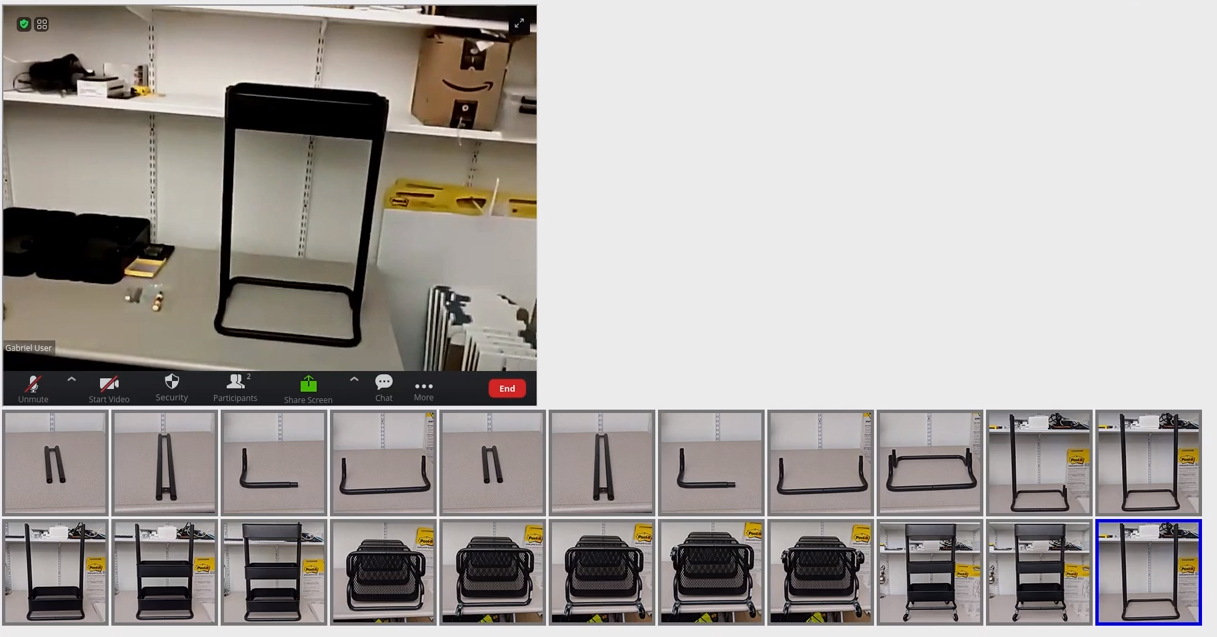
\includegraphics[width=14cm]{figures/expert_ui.png}
  \caption{A screenshot of the web application used by the human task expert.
    The feed from the user's camera is shown on top. The task steps are shown on
    the bottom. The application's current state is the step surrounded by the
    blue box. Clicking on a different step will change the application's state
    to the one that was clicked on.
  }\label{fig:expertui}
\end{figure}

\begin{figure}[h]
  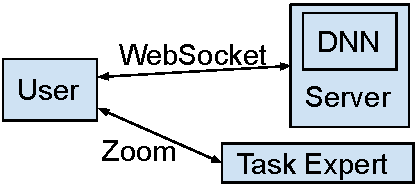
\includegraphics[width=8cm]{figures/human_assitance.pdf}
  \caption{The components of a Gabriel application with human assistance. The
    user primarily receives guidance from a server running a DNN. If the user
    reaches a point where the automated assistance fails, they can switch over
    to receiving guidance from a human expert over a video call.
  }\label{fig:expert_components}
\end{figure}

We connect users to task experts using Zoom, which offers SDKs for several
platforms~\cite{Zoom}. The Gabriel user runs an Android application on a
smartphone, which starts a call with the expert using Zoom's Android SDK.
We plan to develop this application to work on a Google Glass as well.
The human expert uses a web application that incorporates Zoom's Web SDK.
Figure~\ref{fig:expertui} shows a screenshot of this application.
The application works for any WCA task that was created with OpenWorkflow
Editor.
The code can
be modified to use a different video calling service in the future.
The components of the system are shown in Figure~\ref{fig:expert_components}.

\section{Simulating Call Centers}

Supporting a large number of people using WCA applications at the same time
would require multiple human experts answering support calls.
It is important to employ enough experts to ensure that wait times are
reasonable.
However, having too many experts working at one time will create unnecessary
expenses.
The M/M/N model (Erlang-C) is often used to model call centers~\cite{queue1}.
This model assumes that call service times are exponentially distributed.
However, two studies of logs from actual call centers have shown service times
to be lognormally distributed~\cite{queue1, queue2}.
\citet{queue1} examined the expected call center wait time $E(W)$ using the
following approximation for an M/G/N queue:

\[
E(W) \approx \frac{1}{N} \frac{\rho}{1 - \rho} \frac{1 + C_s^2}{2} E(S)
\]

$N$ is the number of agents,
$C_s = \sigma_s / E(S)$ is the coefficient of variation for service, and
$E(S)$ and $\sigma_s$ are the mean and standard deviation of service times

The system occupancy is:
\[
\rho = \frac{\lambda}{N \mu}
\]

$\lambda$ is the arrival rate and $\mu$ is the service rate.

The M/G/N queue assumes that all call inter-arrival times are independent of
service times and other inter-arrival times.
If a user had the option to give up on waiting, this would violate the
independence assumption.

We compared the wait times from this formula with a simple Monte Carlo
simulation that obeys the independence assumption.
The simulation just modeled users calling in, waiting until an expert in the
call center is available to speak, and then the user and the expert are on the
call for a certain amount of time.
There is a single queue for all users waiting for an expert, and it is serviced
in FIFO order.
An expert will service the next call from the queue as soon as they finish their
current call.
The inter-arrival time between calls coming in was sampled from an exponential
distribution.
The lengths of calls were sampled from an exponential distribution with a longer
tail.
These two distributions are depicted in Figure~\ref{fig:simple_sim1_dists}.
Samples were generated using SciPy~\cite{scipy}.
Unfortunately we did not have any real data to help inform the parameter values
for our distributions.
Figure~\ref{fig:simple_sim1_results} shows how the waiting times from our
simulation and the formula vary as we increase the number of experts.
We did not report results with fewer than four experts, because the system
occupancy was above 1.
This means that calls were arriving faster than they could be answered in these
cases, so the queue would continue to grow the longer the simulation was run.

\begin{figure}[h]
  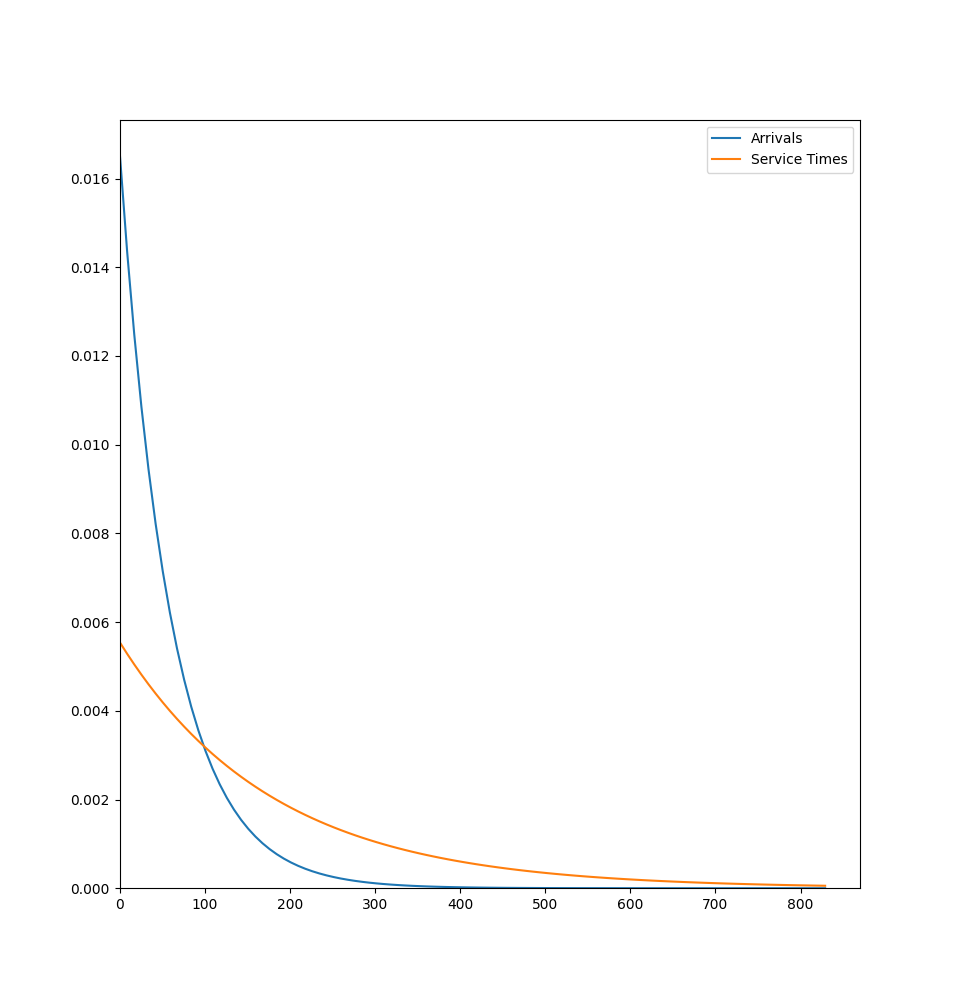
\includegraphics[width=4in]{figures/montecarlo/expon_expon.png}
  \caption{
    The distributions that our first simple simulation sampled times from.
    The inter-arrival times and service times were both sampled from
    exponential distributions.
  }\label{fig:simple_sim1_dists}
\end{figure}

\begin{figure}[h]
  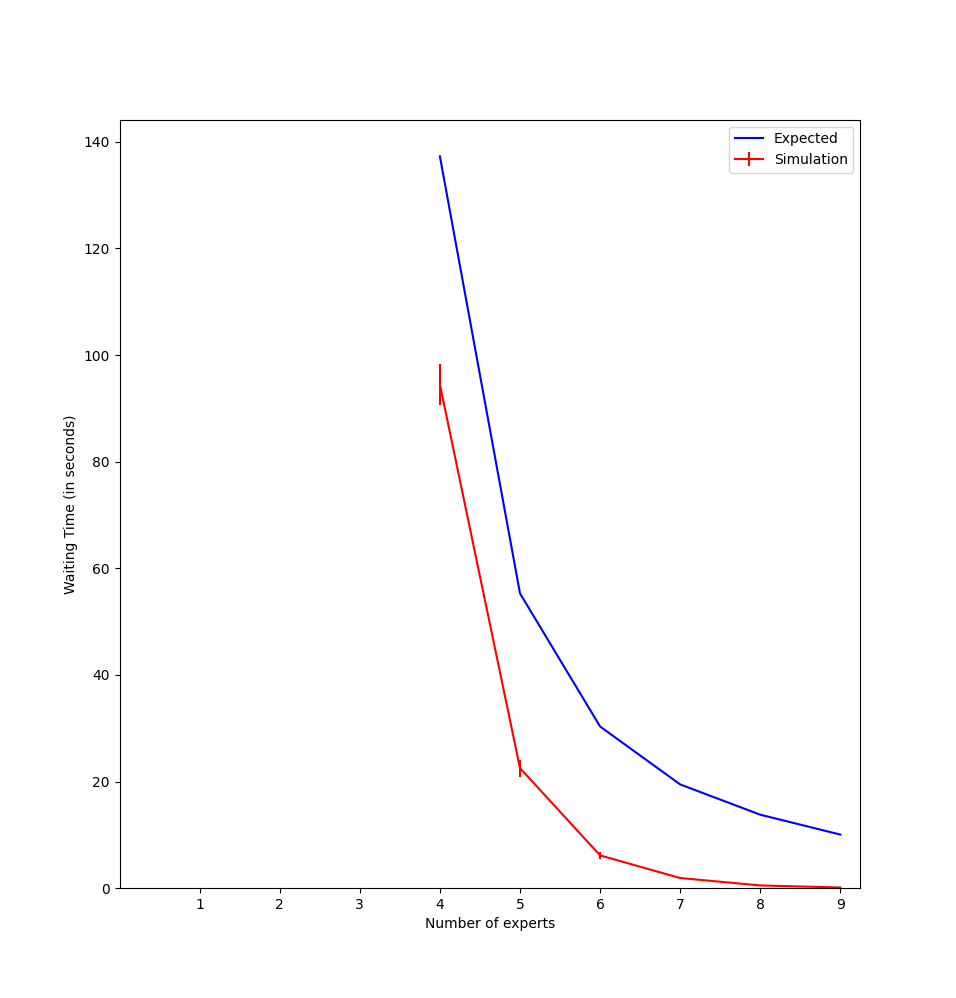
\includegraphics[width=4in]{figures/montecarlo/independent_calls_expon.png}
  \caption{
    The waiting times resulting from our simulation and the approximation
    formula.
    The time values were sampled from the distributions shown in
    Figure~\ref{fig:simple_sim1_dists}.
  }\label{fig:simple_sim1_results}
\end{figure}

We modified our simulation to sample call lengths from a lognormal distribution,
but we kept the exponential distribution for inter-arrival time samples.
The distributions for this version of our simulations are depicted in
Figure~\ref{fig:simple_sim2_dists}.
The results from the simulation and the formula are shown in
Figure~\ref{fig:simple_sim2_results}.

\begin{figure}[h]
  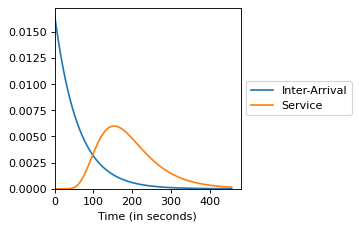
\includegraphics[width=4in]{figures/montecarlo/expon_lognorm.png}
  \caption{
    The distributions that our second simple simulation sampled times from.
    The inter-arrival times were sampled from an exponential distribution.
    The service times were sampled from a lognormal distribution.
  }\label{fig:simple_sim2_dists}
\end{figure}

\begin{figure}[h]
  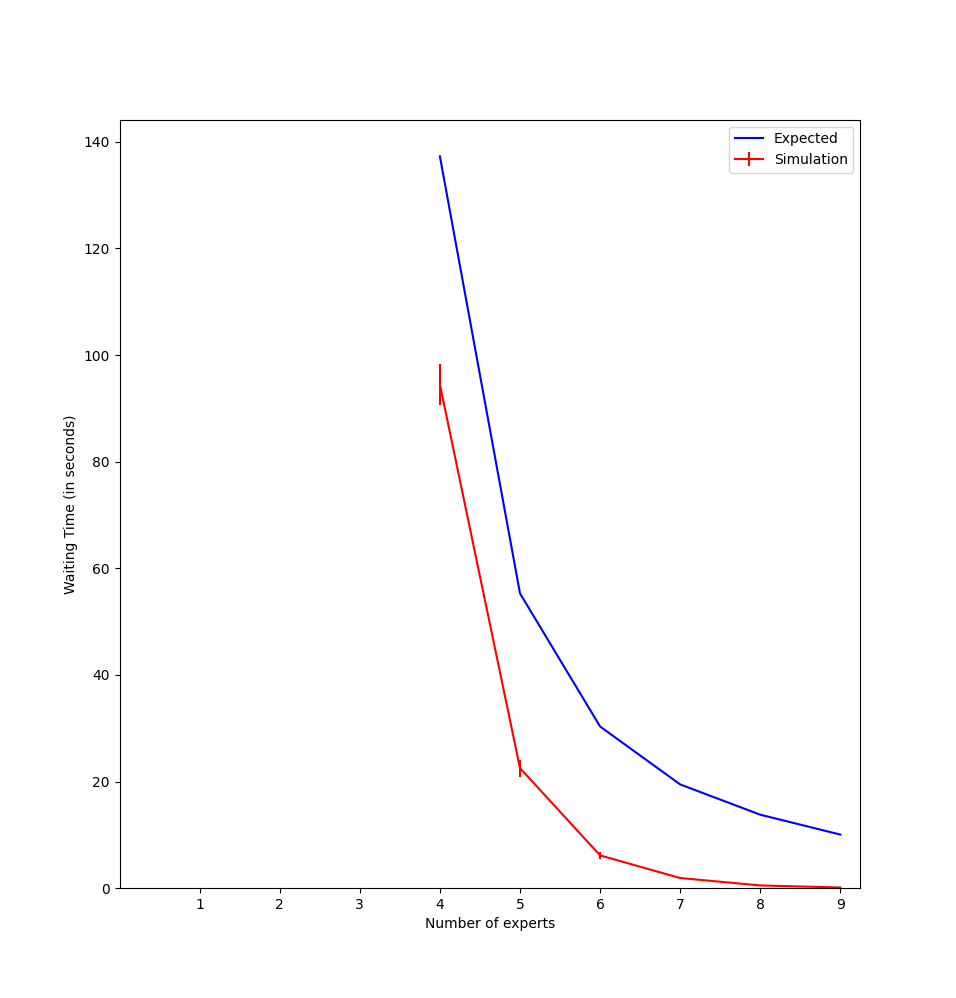
\includegraphics[width=4in]{figures/montecarlo/independent_calls_expon.png}
  \caption{
    The waiting times resulting from our simulation and the approximation
    formula.
    The time values were sampled from the distributions shown in
    Figure~\ref{fig:simple_sim2_dists}.
  }\label{fig:simple_sim2_results}
\end{figure}

The waiting time from the formula was higher than the waiting time from
the simulation in every case.

\subsection{Simulating All Steps}

We expanded our simulation to model users completing an entire task with a WCA
application.
Inter-arrival times for users starting the task are sampled from an exponential
distribution.
The simulation models users completing the task according to the process
described in Figure~\ref{algo:sim}.
This process is repeated for each simulated user.
The simulation allows users to work in parallel.
However, if a user calls for help while all experts are busy, they must wait in
a queue for service.
As in the previous simulations, all users wait in a single queue that is
serviced in FIFO order.

\begin{algorithm}[h]
  \For{Step in task}{
    sample patience length\;
    sample step success\;
    \eIf{step success is 1}{
      sample step length\;
      \eIf{step length < patience length}{
        Pause for step length\;
        User completes step successfully\;
      }{
        Pause for patience length\;
        User calls expert for help\;
        }
      }{
        Pause for patience length\;
        User calls expert for help\;
    }
  }
  \caption{
    The process used to simulate one user completing a task using a WCA
    application.
  }\label{algo:sim}
\end{algorithm}

Patience length is sampled from a generalized Pareto distribution.
\citet{patience} found a generalized Pareto distribution to be a good fit for
samples of time that people waited before crossing streets, while the crossing
signal was telling them not to cross.
Step success was sampled from a Bernoulli distribution.
Step length was sampled from an exponentially modified Gaussian distribution.
The exponentially modified Gaussian distribution is commonly used to model
reaction times~\cite{dawson1988fitting}.
Figure~\ref{fig:step_patience} shows the generalized Pareto and exponentially
modified Gaussian distributions that were used.

When the sampled step success value is 1, and the patience length value is
smaller than the step length value, the user will call the expert for help.
This represents a user giving up on a step that is possible.
One can increase the fraction of steps that a user will give up on by shifting
the step length distribution to the right and/or shifting the patience length
distribution to the left.

\begin{figure}[h]
  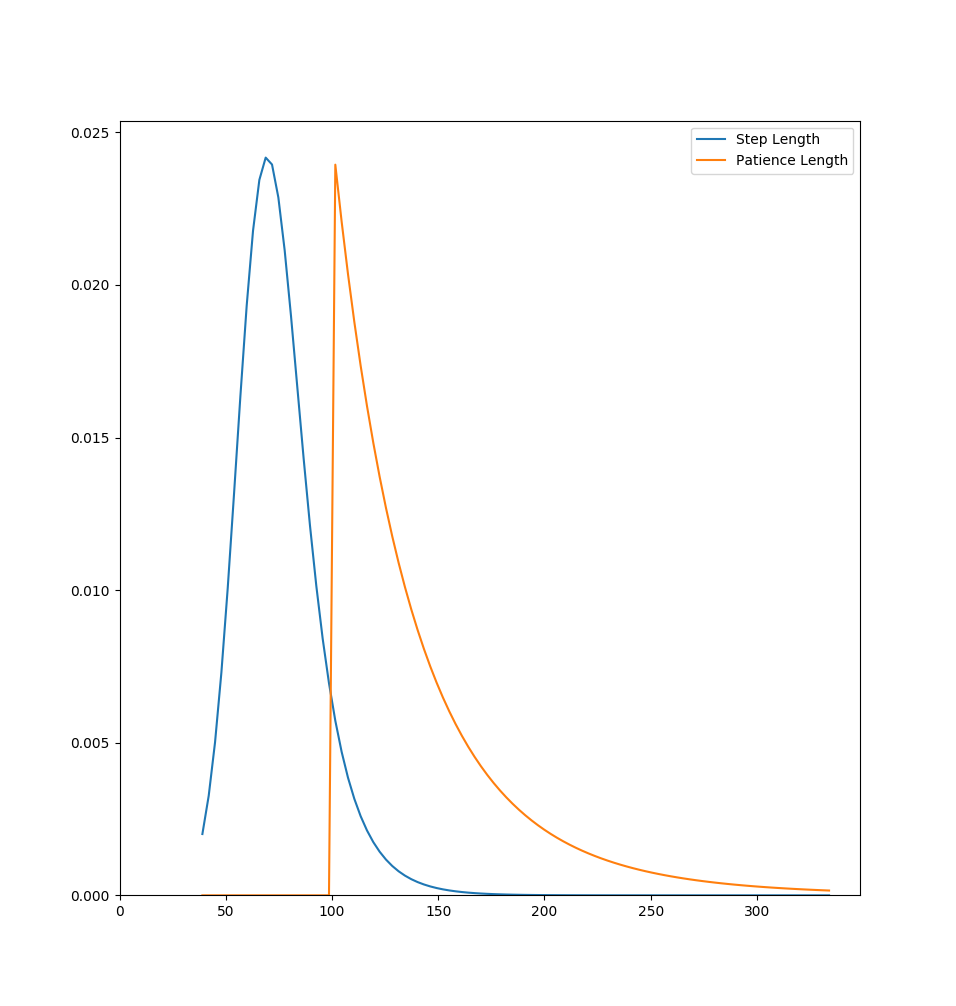
\includegraphics[width=4in]{figures/montecarlo/step_patience.png}
  \caption{
    The generalized Pareto distribution that our simulation samples patience
    length from, and the exponentially modified Gaussian distribution that our
    simulation samples step length from.
  }\label{fig:step_patience}
\end{figure}

The samples from the exponential distribution that were used to determine
Inter-arrival times for users starting the task are shown in
Figure~\ref{fig:arrival_times}.
The times at which a user in our simulation called for help are shown in
Figure~\ref{fig:step_patience}.
We fit an exponential curve to both of these sets of data.
The $R^2$ for the exponential fit was 0.991 for the inter-arrival times of users
starting the task, and 0.986 for the inter-arrival times of users calling for
help.

\begin{figure}[h]
  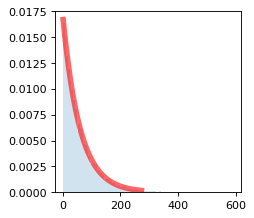
\includegraphics[width=4in]{figures/montecarlo/arrival_times.png}
  \caption{
    Our inter-arrival time samples for users starting the task are shown in
    blue.
    These were drawn from an exponential distribution.
    We fit an exponential curve to this data, which is shown in red.
  }\label{fig:arrival_times}
\end{figure}

\begin{figure}[h]
  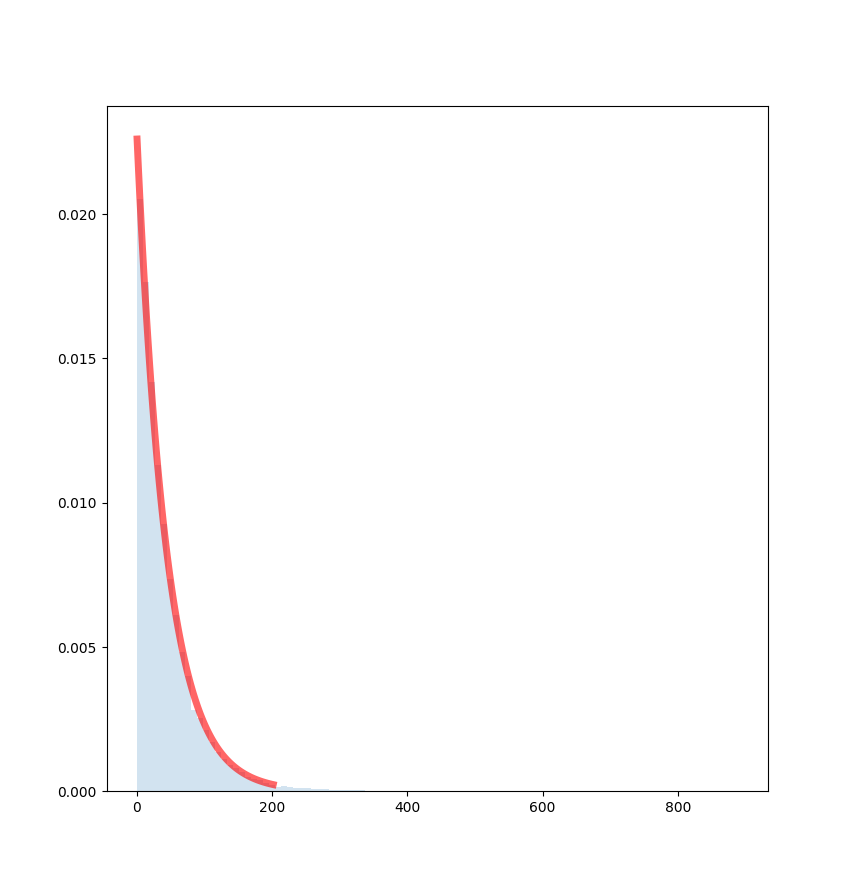
\includegraphics[width=4in]{figures/montecarlo/call_times.png}
  \caption{
    The inter-arrival times for help calls that resulted from our simulation.
    We fit an exponential curve to this data, which is shown in red.
  }\label{fig:step_patience}
\end{figure}

Our simulation sampled call lengths from a lognormal distribution.
The average waiting time for users in our simulation is shown in
Figure~\ref{fig:full_expected_sim}, along with the expected waiting time for an
M/G/N queue.
As with our simple simulations, the waiting time from the formula was slightly
higher than the waiting time from this simulation in every case.
The inter-arrival times for users calling for help are exponentially
distributed, so we expect to see results that are similar to our simple
simulation, where call inter-arrival times were directly sampled from an
exponential distribution.

\begin{figure}[h]
  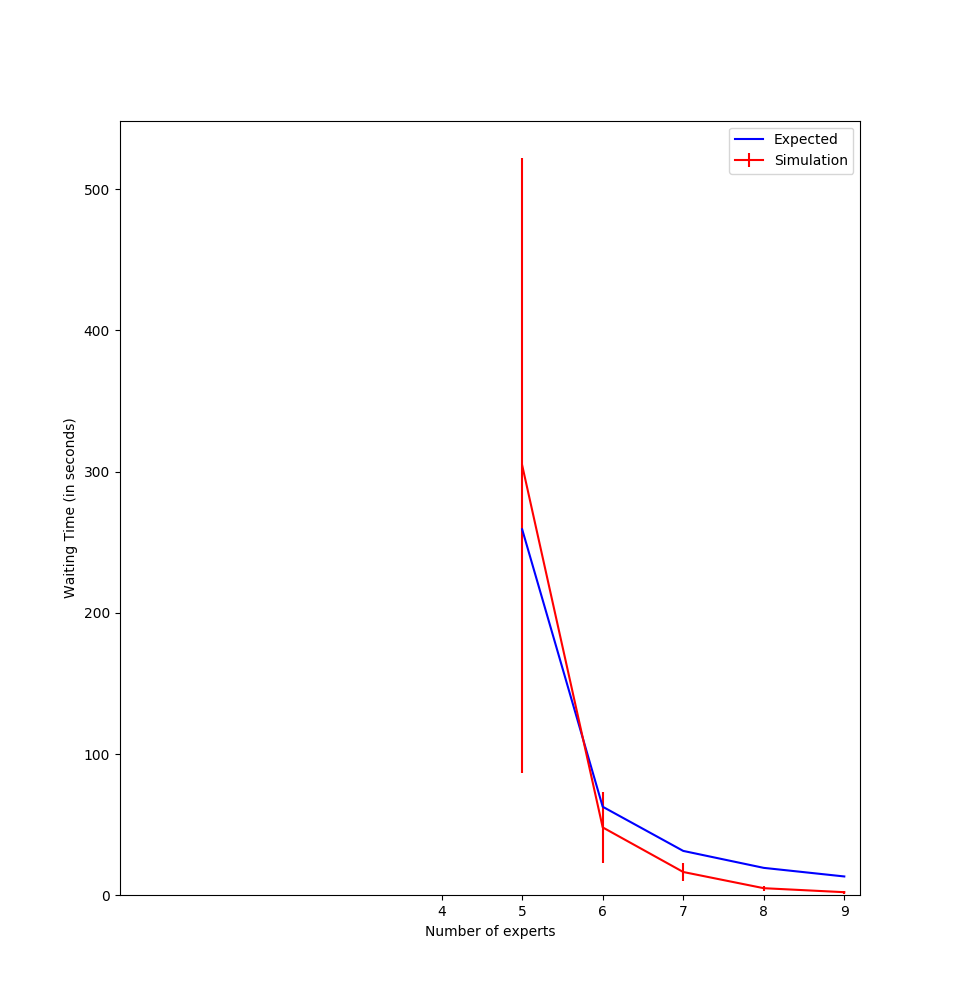
\includegraphics[width=4in]{figures/montecarlo/full_expected_sim.png}
  \caption{
    The average waiting time for simulated users, and the expected waiting time
    for an M/G/N queue.
  }\label{fig:full_expected_sim}
\end{figure}

We ran versions of our simulation with two alternative orderings for servicing
calls.
The first alternative ordering served the user in the queue who has completed
the largest number of steps first.
The next ordering prioritized the user who had been stuck on a step for the
largest amount of time.
In particular, a user who spent three minute trying to complete a step, and then
called the expert one minute ago would get serviced before a user who spent one
minute trying to complete a step, and then called the expert two minutes ago.
A comparison of these queuing strategies is shown in
Figure~\ref{fig:full_three_strategies}.
The results were nearly identical with all three strategies.

\begin{figure}[h]
  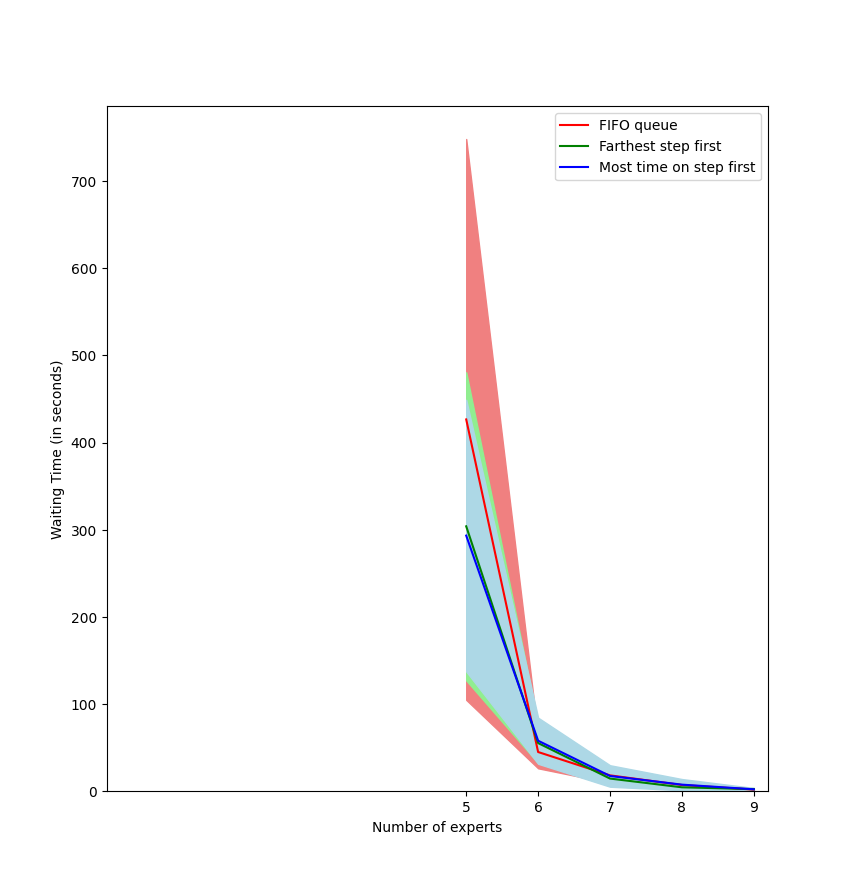
\includegraphics[width=4in]{figures/montecarlo/full_three_strategies.png}
  \caption{
    A comparison of simulation results, with three different queuing strategies.
  }\label{fig:full_three_strategies}
\end{figure}

Our code can easily be modified and re-run with different distributions or
parameters for these distributions.
We did not have any real data to use to set the parameter values of our
distributions.
However, someone running a call center for Gabriel applications could easily
re-run our simulations after finding out these parameter values, in order to
forecast wait times and determine the number of human experts that should be
available to help people trying to complete tasks.
